Im folgenden werden die Notwendigen einstellungen und wie sie ermittelt wurden beschrieben. Dabei wird auf die wichtigen Parameter eingegangen und die verwendeten Werte erläutert. Im folgenden ist die Ordnerstruktur der Simulationen dargestellt, welche von \texttt{OpenFOAM} maßgeblich vorgegeben ist. Der Ordner \texttt{0.orig} enthält die Dateien, die zur initialisierung der Simulation benötigt werden. Bei Beginn der Initialiserung der Simulaiton wird automatisch anhand der Datein in diesem Ordner ein Ordner \texttt{0} erstellt, der die initialisierten Felder enthält, die für die Simulation benötigt werden. Im Ordner \texttt{constant} sind jene Datein, die Physikalische Eigenschaften definieren und wie sie während der Simulation behandelt werden sollen. Im Ordner \texttt{system} sind Dateien, die die Simulation selbst definieren. Unter anderem Die Geometrie und die Vernetzung oder auch dauer der Simulation oder im Falle des diffusen interfaces auch dessen initialisierung. 
\dirtree{%
.1 /.
.2 0.orig.
.3 \ldots.
.2 constant.
.3 \ldots.
.2 system.
.3 \ldots.
} 
Im folgenden werden alle wichtigen einstellungen vorgestellt und gegebenenfalls kurz erläutert. Es wird jedoch davon ausgegangen, dass der Leser mit den Grundlegenden einstellungen von \texttt{OpenFOAM} vertraut ist.

\section{Geometry and Discretization}
Die Geometrie der Kapillare wird so angenommen, dass sie wie in Abbildung \ref{fig: Capillary Geometry} zu sehen, ein Reservoir mit Wasser hat, welches durch Oberflächeneffekte in die Kapillare strömt. Durch die Annahme, dass sich ein Teil des Wassers bereits in der Kapillare befindet, wird in der Simulieren Geometrie lediglich die Randbedingung so gesetzt, dass das Wasser in diesem Reservoir nachströmen kann und das Reservoir nicht mit modelliert und diskretisiert werden muss. Die Dimensionen der Kapillare ergeben sich daraus, dass die Simulation der Kapillare perspektivisch auch mit experimenten verglichen werden soll. Daher wurden auch weitere, komplexere Geometrien simuliert, die jedoch nicht Teil dieser Arbeit sind. 
Wie zu erkennen, handelt es sich um eine Kapillare mit lediglich $6nm$ Durchmesser. Eine Simulation so kleiner Kapillare wurde soweit bekannt bisher nicht mit der Phasenfeld methode Simuliert.


\begin{figure}[h]
    \centering
    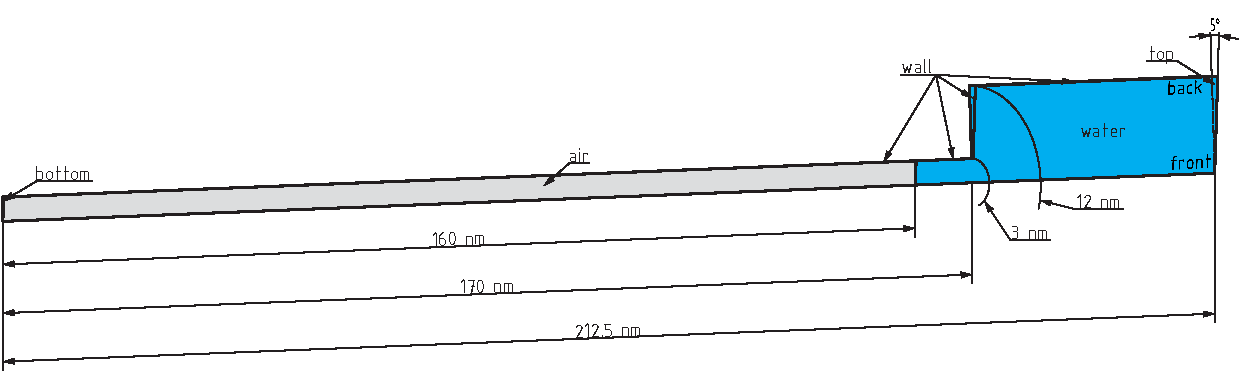
\includegraphics[width=.95\textwidth]{Pictures/Cap_5DEG.pdf}
    \caption{Schematic of used Capillary}
    \label{fig: Capillary Geometry}
\end{figure}
Wie bereits im Bild angedeutet wird nicht die gesamte Kapillare simuliert, sondern lediglich ein segment der Kapillare, \textit{wedge} genannt. Dabei wird angenommen, dass die Strömung in der Kapillare achsensymmetrisch ist, was die Simulation dahingehend stark vereinfacht, dass zur Diskretisierung weniger Elemente benötigt werden, da in diesem Fall nur ein $5^{\circ}$ großes Segment der Kapillare simuliert wird. Eine notwendige Bedingung zur Simulation der Wedge ist es, dass diese nur ein Element in radialer Richtung haben darf. 
Die Diskretisierung der Geometrie wurde so gewählt, dass die Elemente eine Kantenlänge von $0.3nm$ bis $0.4nm$ haben. Aufgrund der duirch die Annahmen, simplen geometrie kann diese ohne weiteres direkt in einer \texttt{blockMeshDict}-Datei definiert werden. Darin wird die Geometrie über Vertices beschrieben und auf blöcke reduziert. Um die Randbedingunen auf den Oberflächen definieren zu können, müssen diese ebenfalls darin definiert und benannt werden. In Abbildung \ref{fig: Capillary Geometry} sind neben der Geometrie auch die Flächen, die mit Randbedingungen versehen wurden benannt. Die Flächen \texttt{front} und \texttt{back} sind sich gegenüberliegende Flächen der Wedge und müssen dementsprechende Ranbedinungen erhalten. Die \texttt{wall} Flächen sind nicht durchdringbare Oberflächen und \texttt{top}, bzw. \texttt{bottom} Oberflächen durch die ein Fluss zugelassen wird. Zur erstellung der \texttt{blockMeshDict}-datei, wurde ein python skript erstellt, welches anhand des Kapillardurchmessers und länge eine Datei mit den in Abbildung \ref{fig: Capillary Geometry} dargestellten Benennungen der Oberflächen erstellt. Für diese müssen Randbedingunen definiert werden, welche in der folgenden Tabelle \ref{tab: BoundaryConditions} aufgelistet sind.

\begin{table}[h]
    \centering
        \caption{relevant boundary conditions wall}
        \label{tab: BoundaryConditions_wall}
        \begin{tabular}{lll}
            Parameter & Value \\ \hline
            orderparameter $C$ & \texttt{equilibriumPhaseContactAngle}     \\
            equilibrium contact angle $\theta_{\mathrm{e}}$ & $15^{\circ}$, $45^{\circ}$, $75^{\circ}$\\
            chemisches Potential $\phi$   & \texttt{zeroGradient}        \\ 
            velocity $\mathbf{u}$ &   $\mathbf{u_{\mathrm{w}}} = 0$\\
            pressure $p$&  \texttt{fixedFluxPressure} \\
        \end{tabular}
\end{table}
Für den Ordnungsparameter $C$ wird die Gleichgewichtsrandbedingung angenommen und der Gleichgewichtskontaktwinkel für jede der drei Simulationen mit dieser Geometrie mit $15^{\circ}$, $45^{\circ}$ bzw. $75^{\circ}$ angegeben. Für weitere Simulationen wurde neben der genannten Gleichgewichtsbedingung \texttt{equilibriumPhaseContactAngle}, auch angenommen, dass ein ungleichgewicht nach \ref{sec: nonEquiBC} herrscht. Dazu muss für die Simulationen die Randbedingung zu \texttt{outOfEquilibriumPhaseContactAngle} geändert und ein Wert für $\Gamma_{\mathrm{w}}$ angegeben werden. 
Der Gradient des chemischen potentials an der Wand wird als null gesetzt, genauso wie die Geschwindigkeit der Wand. Die Ranbedingung für den Druck wird mit \texttt{fixedFluxPressure} so gewählt, dass der Druckgradient so angepasst wird, das der Massenfluss am Rand mit der vorgegebenen Geschwindigkeit an der Wand übereinstimmt. Am ein, bzw. Auslass der Kapillare gilt ebenfalls eine \texttt{zeroGradient} Randbedingungn und ein Druck von $0$ Pa.

Weiter werden für die Simulation Wasser und Luft bei $25^{\circ}$ Celsius als Medium angenommen. Damit folgen die in Tabelle \ref{tab:physicalProperties_CaseSetup} dargestellten Materialeigenschaften. 
\begin{table}[h]
    \centering
    \caption{Physical properties}
    \label{tab:physicalProperties_CaseSetup}
    \begin{tabular}{lll}
    fluid & density $\frac{kg}{m^3}$ & kinematic viscosity $\frac{m^2}{s}$ \\ \hline
    water & $1000$                     & $1.00E-06$                          \\
    air   & $1$                        & $1.00E-05$                          \\ 
    \end{tabular}
    \end{table}
Die Oberflächenspannung für ein Wasser-Luft interface für $25^{\circ}$ Celsius ist mit \(0.072 N/m\) gegeben. The interface thickness \( \epsilon \) was chosen to be approximately \(1.7 nm\) \cite{bagheriInterfacialRelaxationCrucial2022}, corresponding to the physical interface thickness. 
Damit sind alle Einstellungen, die direkt aus der Geometrie oder den Materialien folgt getroffen und es folgen weitere Parameter, die für die Simulation notwendig sind.

\section{Simulationsparameter}
The mobility ($\kappa$) is a factor in the phase-field simulation that is difficult to determine. Jacqmin \cite{jacqmin1999CalculationTwoPhaseNavier} suggested an asymptotic behavior for \( \kappa \) of 
\begin{equation}
    \kappa = \mathcal{O}(\epsilon^{\delta})
\end{equation}
and showed that \( 1 \leq \delta < 2 \). Leider gibt es für die Mobility $\kappa$ und Wandrelaxationsfaktor $\Gamma_{\mathrm{w}}$den bisher keine konkrete Berechnungsmethode. Die tatsache, dass diese parameter phänomenologischer natur sind, macht es schwierig sie vorherzusagen und es gibt lediglich empfehlungen. 
For this work, a value of \( \kappa = 1.6 \times 10^{-18} \) was used. Für den Wand relaxationsfaktor $\Gamma_{\mathrm{w}}$ wurde ein wert von \( \kappa = 5 \times 10^{12} \) verwendet. \todo{CHECK}

Für die Annahme zweier nicht mischbarer FLuide ($mu_{\mathrm{A}}, mu_{\mathrm{B}}$) mit unterschiedlichen Viskositäten wird die Oberflächen interpolierte dynamische laminare viskosität $mu_{\mathrm{f}}$in \texttt{phaseFieldFoam} über drei Viskositätsmodelle Berehcnet. Die wahl des Viskositsmodells kann die Ergebisse maßgeblich beeinflussen \todo{ref to image or chapter}. Die drei Methoden sind $\mu_{\mathrm{f}}^{(S)}$ (seriell/arithmethic), $\mu_{\mathrm{f}}^{(\mathrm{P})}$ (parallel/harmonic) und $\mu_{\mathrm{f}}^{(\mathrm{B})}$ (blended) und definiert als
$$
\begin{aligned}
&\mu_{\mathrm{f}}^{(S)} =\frac{\hat{\overline{c}}_{\mathrm{f}}+1}{2}\:\mu_{\mathrm{B}}-\frac{\hat{\overline{c}}_{\mathrm{f}}-1}{2}\:\mu_{\mathrm{A}},  \\
&\mu_{\mathrm{f}}^{(\mathrm{P})} =\frac{\mu_{\mathrm{A}}\mu_{\mathrm{B}}}{\mu_{\mathrm{f}}^{(\mathrm{S})}},  \\
&\mu_{\mathrm{f}}^{(\mathrm{B})} =\eta_{\mathrm{f}}\:\mu_{\mathrm{f}}^{\mathrm{(P)}}+(1-\eta_{\mathrm{f}})\:\mu_{\mathrm{f}}^{\mathrm{(S)}}.
\end{aligned}
$$
Mit $\eta_{\mathrm{f}}$ als ein blending faktor \cite{holzinger2021DirectNumericalSimulation}. Die Einstellung der verwendeten methode erfolgt nach Wahl der Methode in der \texttt{constant/transportProperties} Datei.

Zur initialisierung des diffusiven Interfaces wird auf die \texttt{funkySetFields} bzw. \texttt{funkySetBoundaryField} Methoden zurückgegriffen. Hier muss die Position und Form des interfaces über eine definierende Funktion angegeben werden. Der verlauf des Ordnungsparamters normal zum Interface wird mit der in Abschnitt \ref{sec: DiffusiveInterface} vorgestellten Gleichung \ref{eq: InterfactialNormalDirProfile} definiert. Da in diesen Simulationen das Interface zu beginn als planar angenommen wird, reicht es nur die Position des Interfaces anzugeben.


\section{Auswertungsmethoden}
Zur Auswertung der Simulation wurde unter anderem die Anwendung \texttt{paraview} verwendet. Alle bilder der Simulation wurden damit erzeugt. Die Auswertung und darstellung abgeleiteter oder berechneter Größen in Diagrammen wurden hingegen mit der python bibliothek \texttt{Matplotlib} erzeugt. Dazu wurde ein skript erstellt, das die Ergebnisse der function obsjects sammelt und gegebenenfalls Berechnungen damit vornimmt. 

Mit hilfe von \textit{function objects} können während der laufenden Simulation daten erfasst werden. \texttt{phaseFieldFoam} liefert bereits einige funktionen zum auslesen der Simulation mit, die auch hier verwendet werden. Diese Müssen in der \texttt{controlDict} datei eingebunden und konfiguriert werden. \todo{maybe name some?}

Beispielsweise wird zur analyse der wirkenden viskosen Kräfte in der Wassersäule, benötigen wir die gesamte viskose dissipationskraft in jener Wassersäule über solche function objects exportiert. Diese erhalten wir, wenn die divergenz des viskosen stress tensors $\tau$ aus Gleichung \ref{eq: NSEChanged} über das Gebiet integrieren
\begin{equation}
    \mathrm{F}_{\mathrm{visc}}^{\mathrm{total}} = \int_{\Omega} \mathrm{f}_{\mathrm{visc}}^{\mathrm{total}} dV = \int_{\Omega} \nabla \cdot \tau dV.
\end{equation}



\subsection{Contact Angle measurement}
\label{sec: CA_Measurement}


Der tatsächliche Kontatkwinkel während der Simulation ist aus vielerlei hinsicht interessant. Zum einen, um festzustellen, in wie fern sich die Simulation über die Zeit entwickelt und dem Glecihgewicht annähert oder aber auch, um wirkende Kräfte bestimmen zu können. Die Messung des Kontaktwinkels ist jedoch nicht trivial \cite{carlson2011DissipationRapidDynamic}. Es gibt mehrere Ansätze die verfolgt werden können. In dieser Arbeit wurden zur Auswertung drei unterschiedliche Ansätze gewählt. Es wird angenommen, dass der Meniskus in der Kapillare ein Kreissegment bildet. Dann kann mit Kenntnis der Position des Interfaces an der Wand und Achse der Kapillare der Kontaktwinkel berechnet werden.
\begin{figure}[h]
    \centering
    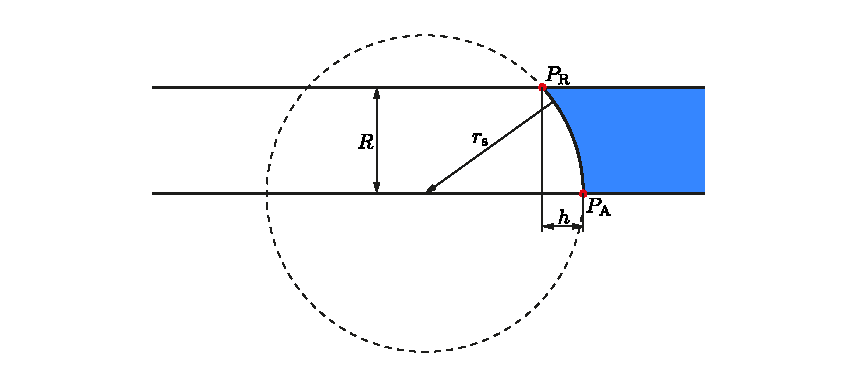
\includegraphics[width=.95\textwidth]{Pictures/RadiusCalc.pdf}
    \caption{Schematic of capillary with relevant dimension for calculation of radius and first Method of contact angle computation}
    \label{fig: RadiusCalc}
\end{figure}
In Abbildung \ref*{fig: RadiusCalc} ist die Geometrie der Kapillare mit den relevanten Größen dargestellt. Die Punkte $P_{\mathrm{R}}$, bzw. $P_{\mathrm{A}}$ sind die Schnittpunkte des Interfaces mit der Kapillarwand und der Rotationsachse. Sind diese Punkte bekannt, kann die höhe $h$ des sphärenabschnitts berechnet werden und damit dann auch der Radius der sphäre $r_{\mathrm{S}}$ mit dem bereits bekannten Kapiilarradius $R$. Die gestrichelte Linie soll dabei verdeutlichen, dass der Radius der sphäre nicht dem der Kapillare entsprechen muss. Zur Berechnung des Kontaktwinkels ist bereits ohne Kenntnis des Radius möglich, wurde aber für spätere berechnungen dennoch bereits eingeführt. Zur Berechnugn des Kontaktwinkels reicht es, die höhe $h$ und den Kapillarradius  zu kennen. Der Kontaktwinkel kann dann mit 
\begin{equation}
    \theta = 90^{\circ}- 2\tan^{-1}\left(\frac{h}{R}\right) 
\end{equation}
berechnet werden. Der Radius ergibt sich aus:
\begin{equation}
    r_{\mathrm{S}} = \frac{R^2}{2h}+\frac{h}{2}.
\end{equation}  

Die beiden weiteren verwendeten Methoden sind im grunde die selben nur, dass unterschiedliche Positionen zur Berechnung des Winkels verwendet werden. Wie in Abbuldung \ref{fig: CA_Method2} gezeigt, wird hier einfach an der Gestrichelten linie Ein schnitt durchgeführt und anschließend ein dreieck gebildet, Womit sich dann der Kontatkwinkel zu
\begin{equation}
    \theta = \tan^{-1}\left(\frac{h_{\mathrm{cut}}}{h}\right)
\end{equation}
ergibt.

\begin{figure}[h]
    \centering
    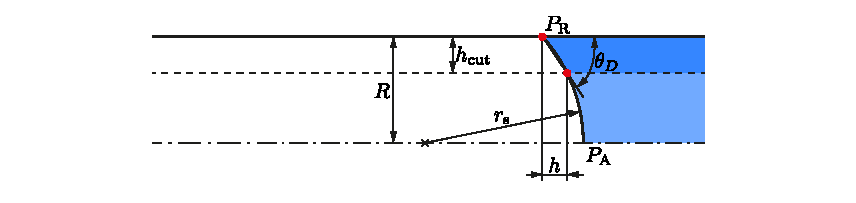
\includegraphics[width=.95\textwidth]{Pictures/CA_CALCMEthod2.pdf}
    \caption{Schematic of capillary with relevant dimension for calculation the second Method of contact angle computation}
    \label{fig: CA_Method2}
\end{figure}


\section{Model Calibration}
Viele der genannten Parameter sind wie bereits erwähnt nur schwer zu definieren. Dher wurden, um diese festlegen zu können Simulationen durchgeführt, bei denen einzele Parameter variiert wurden. Um die notwendige Diskretisierung zu ermitteln wurde eine Netzstudie durchgeführt, für die in Abbildung \ref*{fig: Mesh_Study} die Ergebisse für das Verwendete mesh und für ein feineres Netz mit doppelter Auflösung dargestellt sind. Es wird deutlich, dass die Ergebnisse für die beiden Simulationen übereinstimmen. Das Verwendete Rechennetz besteht damit auf \texttt{4250} Zellen. \todo{image MeshStudy}

\begin{figure}[h]
    \centering
    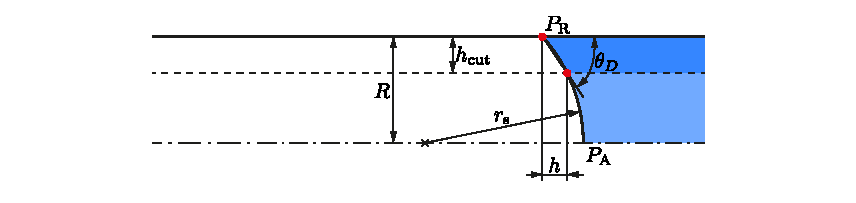
\includegraphics[width=.95\textwidth]{Pictures/CA_CALCMEthod2.pdf}
    \caption{Results of the mesh study for the used and a more refined mesh. Here the imbibition height is plotted over time.}
    \label{fig: Mesh_Study}
\end{figure}
Aufgrund des kleinen Rechennetzes wurde auf die verwendung eins Adaptiv Mesh Refinement verzichtet. 
\todo{Mobility Study}
\todo{evtl gar nciht nennen???}Die Courant zahl ist eine wichtige größe bei den Einstellungen von Simulationen. Daher wurde auch hier anhand mehrerer Simulationen ermittelt 
Um die auswirkungen der unterschiedlichen Viskositätsmodelle beurteilen zu können, wurden auch hier Simulationen durchgeführt. \todo{visc Study and why we used harmonic}
Bei den verwendeten Dimensionen der Kapillare und der Flüssigkeiten, ist zu erwarten, dass der Einfluss der Gravitation vernachlässigbar ist, was auch in gesondert durchgeführten Simulationen gezeigt werden konnte, jedoch aufgrund der geringen aussagekraft einer Darstellung hier nicht weiter gezeigt wird. 

Im zuge dieser Arbeit wurden einige Simulationen und untersuchungen durchgeführt, die schlussendlich nicht weiter verfolgt wurden. Einige dieser Arbeiten waren jedoch auch essentiell, um die Simulationsparameter zu bestimmen. Darunter Simulationen wie die Untersuchung der \textit{mobolity} oder \textit{courant zahl} und der unterschiedlichen \textit{viscosity schemes}. Auch Simulationen mit unterschiedlichen Diskretisierungen des Rechengebiets oder aber auch die verwendung von Adaptiver Netzverfeinerung (AMR) wurden durchgeführt. Es wurden jedoch auch Simulationen durchgeführt, die nicht direkt zur Ermittlung von parametern der Simulation beitragen. Unter anderem Simulationen bei denen der in dieser Arbeit nicht genannte \textit{pinning} Effekt berücksichtigt wurde, oder auch geometrien, die nicht mehr denen dieser Arbeit entsprechen, sondern trotz Vereinfachnungen eher der Realität entsprechen. Diese Simulationen werden in dieser Arbeit jedoch nicht weiter berücksichtigt.  
